\documentclass{article}

\usepackage[final]{style}
\usepackage[utf8]{inputenc} % allow utf-8 input
\usepackage[T1]{fontenc}    % use 8-bit T1 fonts
\usepackage{hyperref}       % hyperlinks
\usepackage{url}            % simple URL typesetting
\usepackage{booktabs}       % professional-quality tables
\usepackage{amsfonts}       % blackboard math symbols
\usepackage{nicefrac}       % compact symbols for 1/2, etc.
\usepackage{microtype}      % microtypography
\usepackage{verbatim}
\usepackage{graphicx}       % for figures
\usepackage{float}
\usepackage{amsmath}

\title{Lecture \#5: Edge detection}

\author{
  Stephen Konz, Shivaal Roy, Charlotte Munger, Christina Ramsey, Alex Iyabor Jr \\
  Department of Computer Science\\
  Stanford University\\
  Stanford, CA 94305 \\
  \texttt{\{swkonz, shivaal, cmunger, cmramsey, aiyabor\}@cs.stanford.edu} \\
}

\begin{document}

\maketitle


\section{Continuing from Last Lecture}
\subsection{Linear Systems}
Linear Systems (Filters) form new images, the pixels of which are a weighted sum of select groupings of the original pixels. The use of different patterns and weights amplifies different features within the original image. A system  $S$ is a linear system If and Only If it satisfies the Superposition Property of systems:
\begin{center}
$S[\alpha f_i[n,m] + \beta f_j[h,m]]$ $=$ $\alpha S[f_i[n,m]] + \beta S[f_j[h,m]]$
\end{center}

As previously introduced in the last lecture, the process of applying a filter to an input image is referred to as \textit{convolution}.

\subsection{LSI (Linear Shift Invariant Systems) and the impulse response}
A shift invariant system is one in which shifting the input also shifts the output an equal amount. A linear shift-invariant (LSI) system's is characterized by its response to an impulse; this response is known as the \textit{impulse response}. The impulse response helps us to understand the output of an LSI system for any given input signal.

\subsection{Why are Convolutions Flipped?}
Proof of $2D$ cross correlation's commutativity:
\begin{align*}
f[n,m] * * h[n,m] &= \sum_{k}^{} \sum_{l}^{} f[k,l] \cdot h[n-k,m-l]\\
\text{let $N = n - k$, $M = m-l$ so $k = n - N$ and $l = m - M$} \\
&= \sum_{k}^{} \sum_{l}^{} f[n-N, m-M] \cdot h[N,M]\\
&= \sum_{N}^{} \sum_{M}^{} h[N,M] \cdot f[n-N, m-M]\\
% &= \sum_{k}^{} \sum_{l}^{} f[n-k,m-l] \cdot  h[k,l] &\\
&= h[n,m] * * f[n,m]
\end{align*}
\subsubsection{Example}
Apply kernel k to matrix M.
$$ M = \begin{bmatrix}
0 & 0 & 0\\
0 & 1 & 0\\
0 & 0 & 0
\end{bmatrix}, \\
k = \begin{bmatrix}
x_{1,1} & x_{1,2} & x_{1,3} \\
x_{2,1} & x_{2,2} & x_{2,3}\\
x_{3,1} & x_{3,2} & x_{3,3}\\
\end{bmatrix}$$
$$ M * k = \begin{bmatrix}
x_{3,3} & x_{3,2} & x_{3,1} &\\
x_{2,3} & x_{2,2} & x_{2,1} &\\
x_{1,3} & x_{1,2} & x_{1,1} &\\
\end{bmatrix}$$
Here, the kernel is expected to match the convolution. Instead, the output is equal to the kernel flipped in the x and y direction. To rectify this, the kernel is flipped at the initial step to ensure correct output form.
\subsection{Convolution vs Cross Correlation}
A convolution is an integral that expresses the amount of overlap of one function as it is shifted over another function. We can think of the convolution as a filtering operation. \newline

The \textit{Correlation} calculates a similarity measure for two input signals (e.g., two image patches). The output of correlation reaches a maximum when the two signals match best. Correlation can be though of as a measure of relatedness of two signals.

\section{Edge Detection in Mammals}

\subsection{Hubel \& Wiesel}
In a series of experiments conducted by Hubel and Wiesel \cite{hubel1960receptive}, the neuron responses in a cat's brain were recorded to observe how each part of the brain responds to different stimuli. They revealed that the cat’s neurons were most excited by the edges at different orientations; namely, certain neurons correlated to specific orientations of edges or edges that moved in specific directions. Having one of these edges moving in its field of vision would cause that particular neuron to fire excitedly.

\begin{figure}[H]
\centering
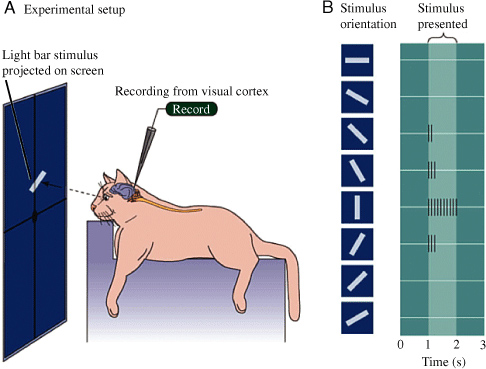
\includegraphics[width=8cm]{hubel_wiesel_cat.jpg}
\caption{The Hubel and Wiesel's experiment. Source: \cite{hubel1960receptive}; Lecture 5, slide 34}
\end{figure}

\subsection{Biederman}
Biederman investigated the rate at which humans can recognize the object they're looking at. To test this, he drew outlines of common and recognizable objects and split them into two halves, with each line segment divided in only one of the halves. These outlines were then shown to partipants to test whether they could recognize the original objects while only seeing half of the original outline. \newline

Surprisingly, he observed no difference in terms of the speed with which people recognized the objects. It was easy for them to recognize an object via only parts of its edges. This study benefits computer vision by providing an insight: even if only part of the original image is shown, a system theoretically should still be able to recognize the whole object or scene.

\begin{figure}[H]
\centering
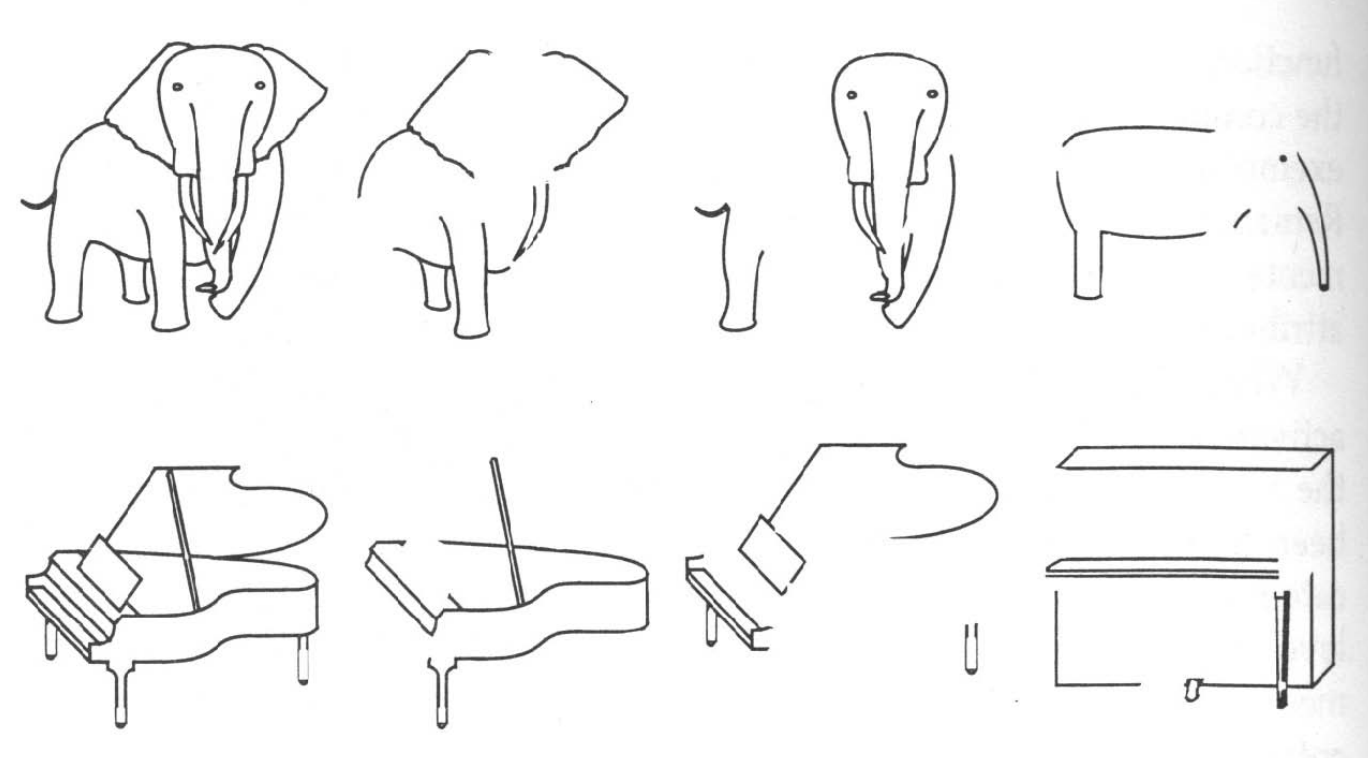
\includegraphics[width=8cm]{biederman_outlines.png}
\caption{The examples of the Biederman's outlines. Source: Lecture 5, slide 36}
\end{figure}

\subsection{Walther, Chai, Caddigan, Beck \& Fei-Fei}
In similar experiments, another group of researchers took two variations of the same image - the original color image and the outline of that image - to test color image vs line image recognition in humans. They traced recognition through different layers, each one a different level of processing in the visual pcortex of the brain. They found that lower layers could recognize the scenes faster via the line image, but as it moved up the layers of the brain (which encode increasingly higher level concepts), the color drawings were much more helpful in allowing people to recognize the scene as compared to the line drawing. This is believed to have happened because lower layers are better at recognizing pieces, like edges, while higher layers are better at recognizing concepts (like "human," "chair," or "tiger").

\begin{figure}[H]
\centering
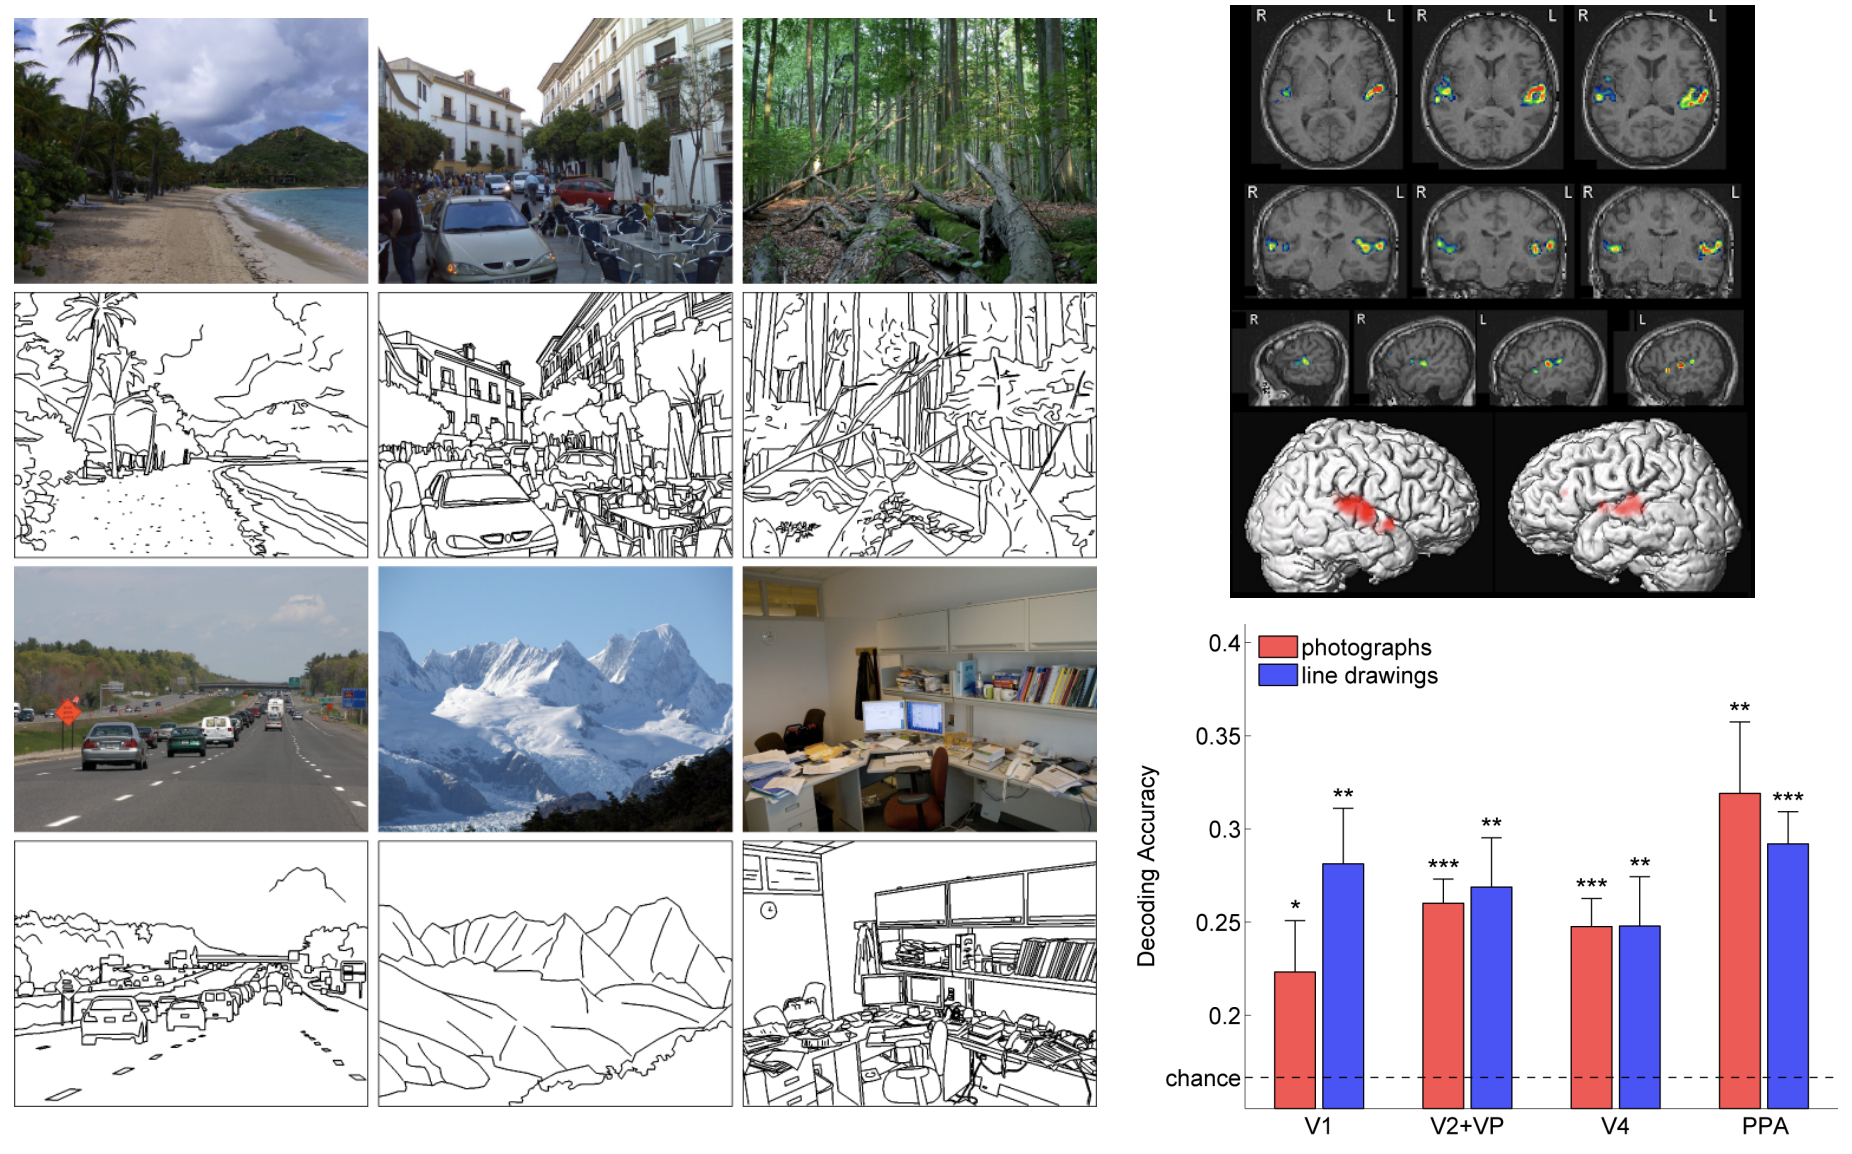
\includegraphics[width=8cm]{fei-fei_images.png}
\caption{The visualization of the images and outcomes. Source: \cite{walther2011simple};Lecture 5, Slide 37}
\end{figure}


\section{Edge Detection for Computer Vision}
The goal of edge detection is to identify sudden changes (\textit{discontinuities}) in an image. Intuitively, most semantic and shape information from the image can be encoded in its edges. \newline

The edges help us extract information, recognize objects, and recover geometry and viewpoint. They arise due to discontinuities in surface normal, depth, surface color, and illumination . \newline

\subsection{Types of Discrete Derivative in 1D}
There are three main types of derivatives that can be applied on pixels. Their formulas and corresponding filters are:\\
Backward
$$\frac{df}{dx} = f(x) - f(x-1) = f'(x)$$
$$[0, 1, -1]$$
Forward:
$$\frac{df}{dx} = f(x) - f(x+1) = f'(x)$$
$$[-1, 1, 0]$$
Central:
$$\frac{df}{dx} = f(x+1) - f(x-1) = f'(x)$$
$$[1, 0, -1]$$
\subsection{Discrete Derivative in 2D}
Gradient vector
$$ \nabla f(x,y) = \begin{bmatrix} f_x\\
f_y\\
\end{bmatrix}  $$
Gradient magnitude
$$ |\nabla f(x,y)| = \sqrt{f_x^2 + f_y^2}$$
Gradient direction
$$ \theta = tan^{-1}\Big( \frac{\frac{df}{dy}}{\frac{df}{dx}}\Big)$$

\subsection{Example}
The gradient at a matrix index can be approximated using neighboring pixels based on the central discrete derivative equation expanded to $2D$. A filter like
$$ \frac{1}{3}\begin{bmatrix} -1 & 0 & 1\\
-1 & 0 & 1 \\
-1 & 0 & 1 \\\end{bmatrix}$$
When overlapped on top of a pixel $x[m,n]$, such that the center of the filter is located at $x[m,n]$ shown with its neighbors below
$$ \begin{bmatrix}
...&...&...&...&...\\
...&x_{m-1,n-1} & x_{m-1,n} & x_{m-1,n+1}&... \\
...&x_{m,n-1} & x_{m,n} & x_{m,n+1}&...\\
...&x_{m+1,n-1} & x_{m+1,n} & x_{m+1,n+1}&...\\
...&...&...&...&...\\
\end{bmatrix}
$$
Produces an output of
$$\frac{1}{3}\Big((x_{m-1,n+1} - x_{m-1,n-1})+ (x_{m,n+1}-x_{m,n-1}) + (x_{m+1,n+1} - x_{m+1,n-1})\Big) = $$
Which is equivalent to an approximation of the gradient in the horizontal ($n$) direction at pixel $(m,n)$. This filter detects the horizontal edges, and a separate kernel is required to detect vertical ones.

\section{Simple Edge Detectors}

\subsection{Characterizing Edges}
Characterizing edges (i.e., characterizing them properly so they can be recognized) is an important first step in detecting edges. For our purposes, we will define an edge as a rapid place of change in the image intensity function. If we plot the intensity function along the horizontal scanline, we see that the edges correspond to the extra of the derivative. Therefore, noticing sharp changes along this plot will likely give us edges.

\begin{figure}[H]
\centering
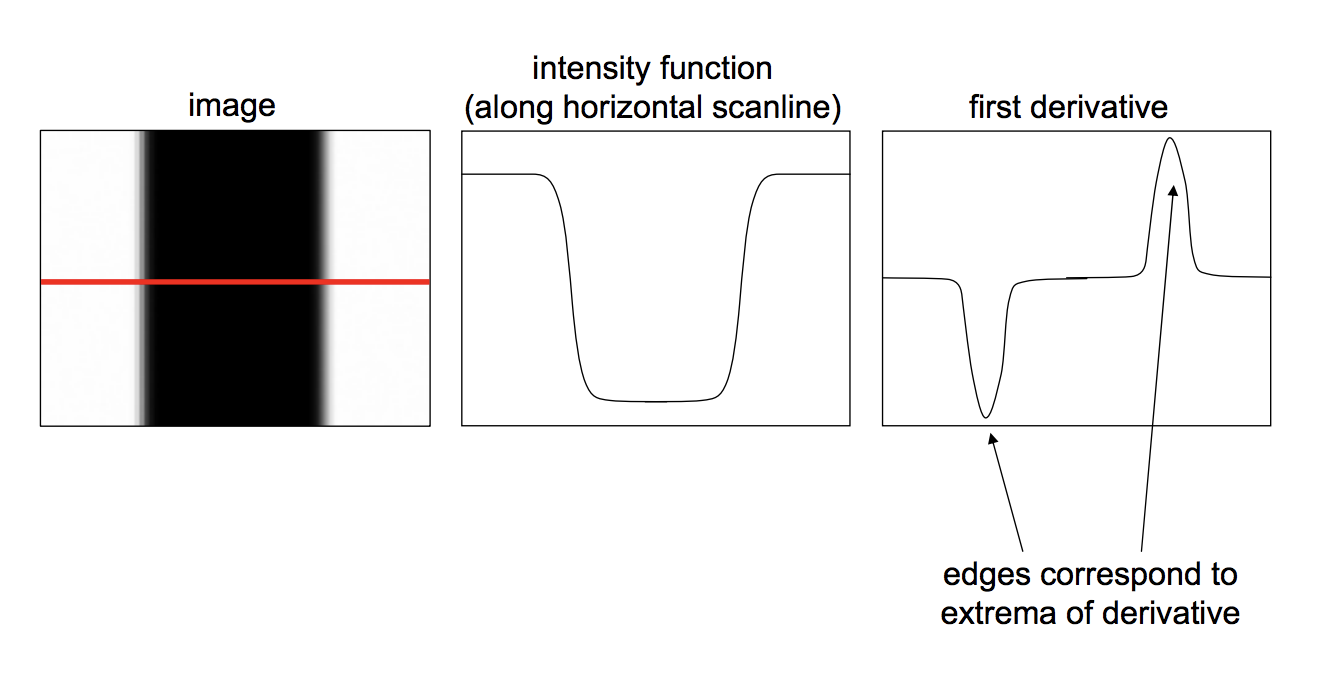
\includegraphics[height=4cm]{lazebnik.png}
\caption{An image with intensity function and first derivative. Source: Lecture 5, slide 66}
\end{figure}

\subsection{Image Gradient}
The gradient of an image has been defined as the following:
$$\nabla f = \left[ \frac{\partial f}{\partial x}, \frac{\partial f}{\partial y}\right],$$
while its direction has been defined as:
$$\theta = \tan^{-1} \left( \frac{\partial f}{\partial y} / \frac{\partial f}{\partial x} \right).$$


\begin{figure}[H]
\centering
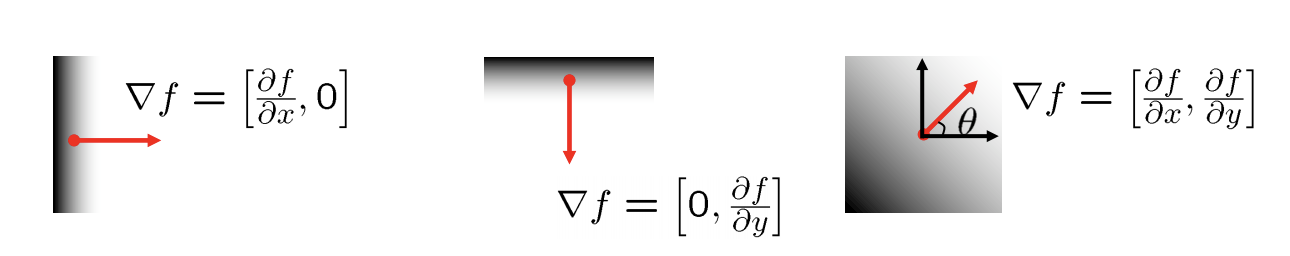
\includegraphics[width=10cm]{seitz_gradient_direction.png}
\caption{The gradient vector directions. Source: Lecture 5, slide 67}
\end{figure}

The gradient vectors point toward the direction of the most rapid increase in intensity. In vertical edge, for example, the most rapid change of intensity occurs in the $x$-direction.

\begin{figure}[H]
\centering
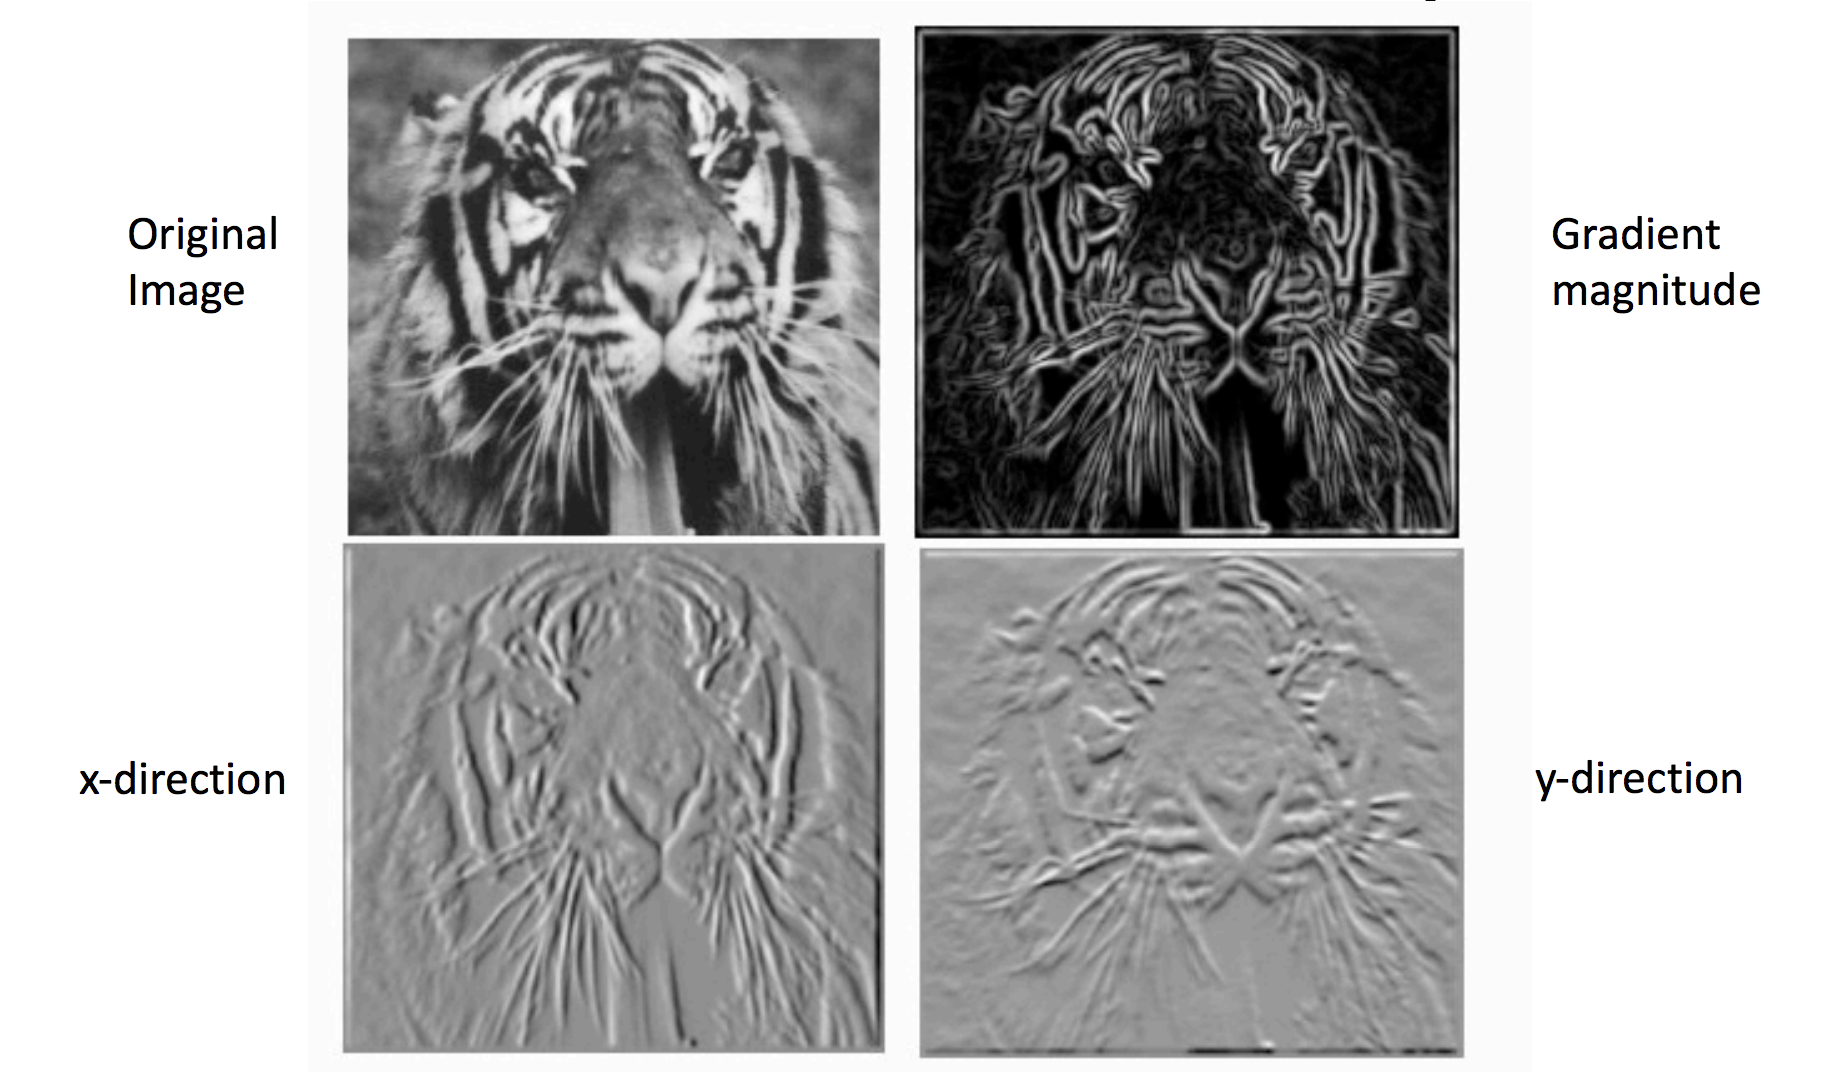
\includegraphics[width=10cm]{lazebnik_tiger.png}
\caption{The gradients as applied to the image of a tiger. Source: Lecture 5, slide 68}
\end{figure}

\subsection{Effects of Noise}

If there is excessive noise in an image, the partial derivatives will not be effective for identifying the edges. \newline

\begin{figure}[H]
\centering
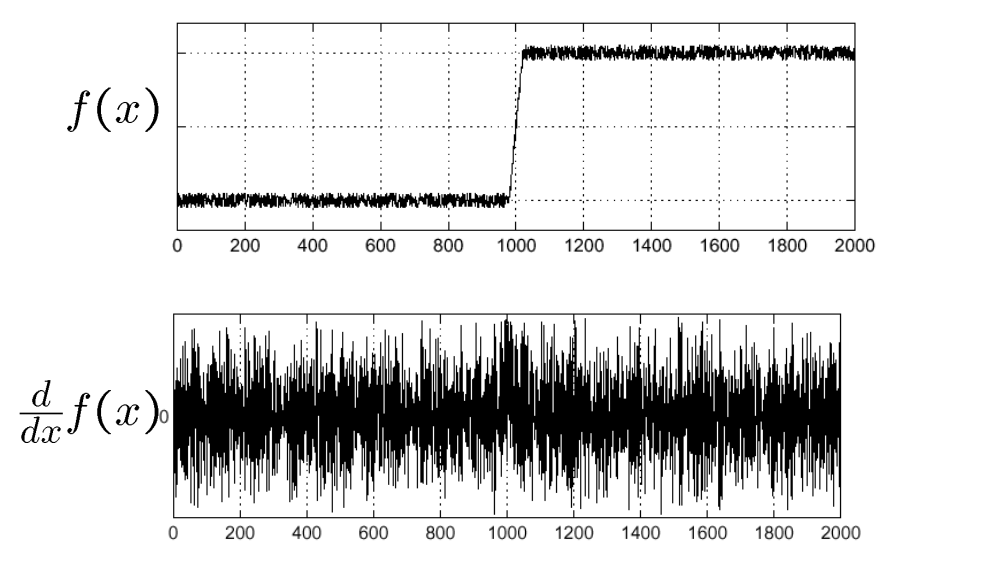
\includegraphics[width=10cm]{seitz_noise.png}
\caption{The derivative of an edge in a noisy image. Source: Steve Seitz; Lecture 5, slide 70}
\end{figure}

In order to account for the noise, the images must first be smoothed. This is a process in which pixel values are recalculated so that they more closely resemble their neighbors. The smoothing is achieved by means of convolving the image with a filter (e.g., gaussian kernel). \newline

There are, of course, some concerns to keep in mind when smoothing an image. The image smoothing does remove noise, but it also blurs the edges; the use of large filters can result in the loss of edges and the finer details of the image.

\begin{figure}[H]
\centering
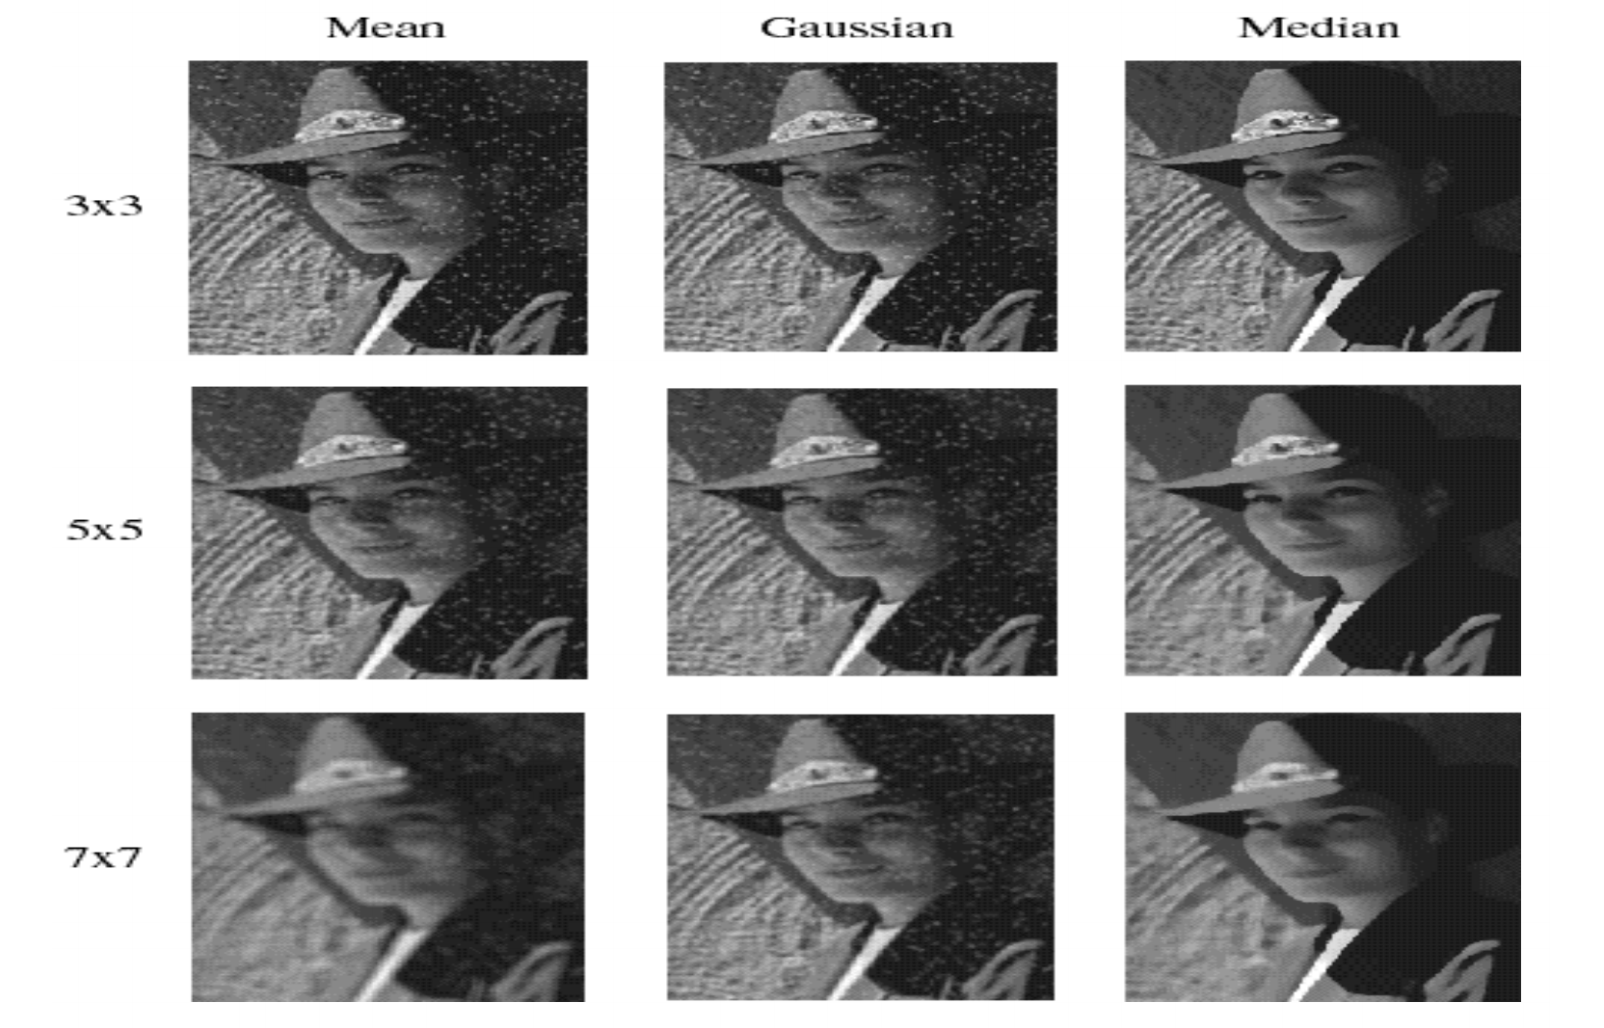
\includegraphics[width=10cm]{seitz_smoothing.png}
\caption{Smoothing with different filters and filter sizes. Source: Steve Seitz; Lecture 5, slide 75}
\end{figure}


The image smoothing facilitates the process of edge detection. After smoothing an image $f$, the search for peaks is initiated by calculating $f * \frac{d}{dx}g$ with kernel $g$.

\subsection{Gaussian Blur}

The Gaussian blur is the result of blurring an image by a Gaussian function to reduce image noise. It is a low-pass filter, meaning it attenuates high frequency signals. You will generally use Gaussian blurring as a preliminary step.
\newline
One dimension:
$$G(x) = \frac{1}{\sqrt{2\pi\sigma}}e^{-\frac{x^2}{2\sigma^2}}$$
Two dimension:
$$G(x,y) = \frac{1}{2\pi\sigma}e^{-\frac{x^2+y^2}{2\sigma^2}}$$


\section{Designing a Good Edge Detector}
An optimal edge detector must have certain qualities:
\begin{enumerate}
    \item Good detection
    \begin{itemize}
        \item It must minimize the probability of detecting false positives (which are spurious edges, generally caused by noise) and false negatives (missing real edges, which can be caused by smoothing, among other things). If it detects something as an edge, it should be an edge.
    \end{itemize}
    \item Good localization
    \begin{itemize}
        \item The detected edges must be as close as possible to the actual edges in the original image. The detector must identify where the edges occur and pinpoint the exact location of the edge; it must also be consistent in determining which pixels are involved in each edge.
    \end{itemize}
    \item Silent response
    \begin{itemize}
        \item It must minimize the number of local maxima around the true edge (returning one point only for each true edge point). It should tell you that there is one very specific edge instead of splitting one edge into multiple detected edges. In other words, only the real border of the edge is captured; other possibilities are suppressed.
    \end{itemize}
\end{enumerate}

\begin{figure}[H]
\centering
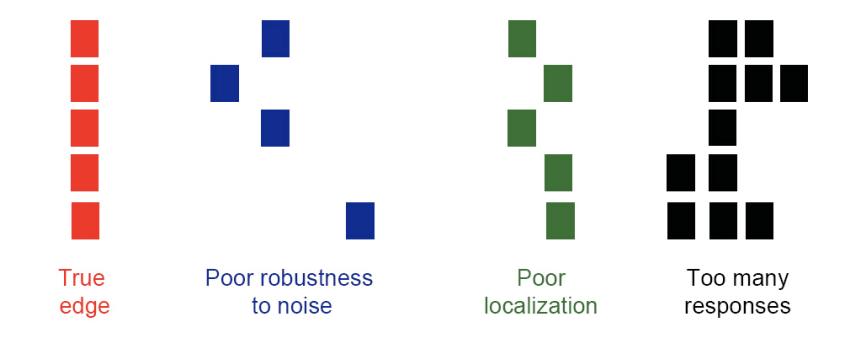
\includegraphics[width=8cm]{fei-fei_detection.png}
\caption{Sample problems of bad edge detectors. Source: Lecture 5, slide 84}
\end{figure}



\small
\bibliographystyle{plain}
\bibliography{bibliography}
\end{document}
